\chapter{Discovering (Setting Limit for) \Bmumumu at LHCb}
\label{chap:sel}

\textit{LHCb's flagship analyses contain several muons in the final state coming from differently flavoured $B$ mesons. Despite being in this category, search for \Bmumumu is limited by the rareness of its occurence as well as different backgrounds that can mimique its signature in the detector. Moreover, presence of invisible neutrino does induce uncertainties into reconstruction. This \autoref{chap:sel} will concentrate on characterisation of backgrounds as well as selection that is performed in order to reduce the backgrounds.}


\section{Topology of at LHCb \Bmumumu at LHCb}

Upon hadronisation of $b\bar{b}$ pair \Bpm particle will travel less than a milimetre in the laboratory frame of reference before it decays into its decay products. This allows reconstruction of a primary vertex \Gls{PV} and its decay vertex, \textit{secondary vertex} \Gls{SV}. By joining these vertices, direction as well as lenght of the \Bpm existence, also known as flight distance (\Gls{FD}), can be established. In order to infer information about kinematic properties of \Bpm, the decay products are studied. All three muons are used to reconstruct the visible four-momentum. By conservation of momentum with respects to the direction of the flight of \Bpm, neutrino is assigned all missing momentum transverse to the direction of the flight of \Bpm. The schematic diagram can be seen in \autoref{fig:sigtopolog}.

\begin{figure}[!h]
	\centering
	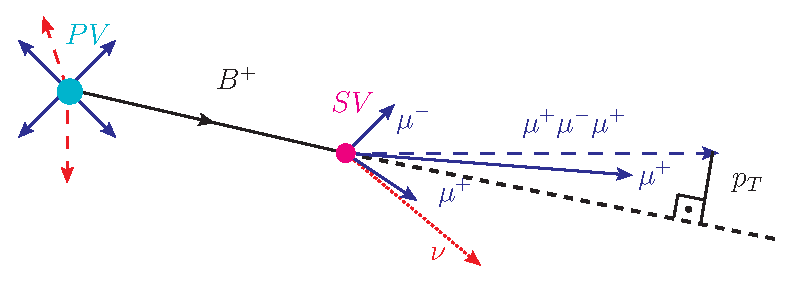
\includegraphics[width = 0.8\textwidth]{figs/sel/DecReco_fin.eps}
	\caption{Schematic view of \Bmumumu decay. At $pp$ interaction point, or $PV$, $b\bar{b}$ pair hadronizes into \Bpm. \Bpm flies some distance before decaying into three muons and neutrino. All charged tracks (in filled-blue) seen can be combined into four-vector representing the visible part of the decay (semifilled-blue). Information about invisible neutrino (semifilled-red) are deduced from the conservation of momentum with respect to the direction of the flight of \Bpm. Neglecting momentum component parallel to the direction of flight for neutrino, transverse component of momentum is given.}
	\label{fig:sigtopolog}
\end{figure}

Altogether it allows for reconstruction of a quantity, \textit{corrected mass}, that plays similar role to invariant mass in fully reconstructed decays. Invariant mass is ususally used in \Gls{LHCb} for fitting distribution from which physics results are extracted as it distinguishes well signal from background and there is minimal modelling problem.

\textit{Corrected mass} is defined as

\begin{equation}
	M_{corr} = \sqrt{{M}^{2} + |p^{2}_{T}|} + |p_{T}|,
\end{equation}	
where the $M^{2}$ is the invariant visible mass squared and $p^{2}_{T}$ is the missing momentum squared transverse to the direction of $B^{+}$ flight.

%\begin{equation}
%M_{B_{corr}} = \sqrt{M_{\mu^{+} \mu^{-} \mu^{+}}^{2} + |p_{T}|} + |p_{T}|,
%\end{equation}	

$M_{corr}$ can be thought of as the the minimal correction to the visible mass to account for the missing neutrino information. The resolution on the \textit{corrected mass} hence becomes a critical quantity that needs to be understood. As the method of reconstruction of corrected mass relies heavily on the knowledge of \Bpm flight direction, the resolution of \Gls{PV} position and \Gls{SV} vertex is crucial. Let $\vec{{x}}_{PV}=\{x_{PV},y_{PV},z_{PV}\}$, $\vec{{x}}_{SV}=\{x_{SV},y_{SV},z_{SV}\} $ be \Gls{PV} and \Gls{SV} vertex position and $\vec{p}=\{E,p_{x},p_{y},p_{z}\}$ be the visible trimuon four-momentum. Then the missing transverse momentum to the direction of the flight $p_{T}$ (momentum of the neutrino) is


\begin{equation}
	p^{2}_{T} = |\vec{p} - (\vec{{x}}_{SV}-\vec{{x}}_{PV})\frac{\vec{p} \cdot(\vec{{x}}_{SV}-\vec{{x}}_{PV})}{|(\vec{{x}}_{SV}-\vec{{x}}_{PV})|^{2}}|^{2}
\end{equation}

In general in order to propagate error on $f(x,y,z)$, where $x,y,z$ are independent variables, the variance of $f(x,y,z)$

\begin{equation}
\begin{aligned}
	\langle f^{2}-\langle f \rangle^{2} \rangle  &=  \langle f(x+\delta x, y+\delta y, z+\delta z)^{2} - f(\langle x \rangle, \langle y \rangle, \langle z \rangle)^{2} \rangle \\
\end{aligned}
\end{equation}

Using first order Taylor expansion of variance and rewriting into the matrix form:

\begin{equation}
\begin{aligned}
%	\langle \frac{\partial{f}}{\partial{x}}  \frac{\partial{f}}{\partial{x}} \times \delta x^{2} + \frac{\partial{f}}{\partial{y}}  \frac{\partial{f}}{\partial{y}} \times \delta y^{2} + \frac{\partial{f}}{\partial{z}}  \frac{\partial{f}}{\partial{z}} \times \delta z^{2} + \sum_{i,j=1..3, i \neq j} \partial_{d_{i}} \partial_{d_{i}}  \frac{\partial{f}}{\partial{x}} \frac{\partial{f}}{\partial{y}} \rangle \\ 
%        = 
       \begin{bmatrix}
		\frac{\partial{f}}{\partial{x}} & \frac{\partial{f}}{\partial{y}} & \frac{\partial{f}}{\partial{z}} \\
       \end{bmatrix}
       \begin{bmatrix}
	       {\delta x}^{2} & \delta x \delta y & \delta x \delta z  \\ 
	        \delta y \delta x & {\delta y}^{2} & \delta y \delta z  \\
	        \delta z \delta x & \delta z \delta y & {\delta z}^{2}  \\
       \end{bmatrix}
       \begin{bmatrix}
		\frac{\partial{f}}{\partial{x}} \\ \frac{\partial{f}}{\partial{y}} \\\frac{\partial{f}}{\partial{z}} \\
       \end{bmatrix}
\end{aligned}
\end{equation}

So now assuming that $x=\vec{{x}}_{PV}$, $y=\vec{{x}}_{SV}$ and $z=\vec{p}$,

\begin{equation}
\begin{aligned}
       \nabla^{T}_{x_{PV}} \rm{COV_{x_{PV}}} \nabla_{x_{PV}} + \nabla^{T}_{x_{SV}} \rm{COV_{x_{SV}}} \nabla_{x_{SV}} + \nabla^{T}_{p} \rm{COV_{p}} \nabla_{p}
\end{aligned}
\end{equation}

where \rm{COV} is the covariance matrix.

In conclusion in order to calculate error on \textit{corrected mass}, $\delta_{corrm}$


\begin{equation}
\begin{aligned}
	\delta_{corrm} = \sqrt{ \langle f^{2}-\langle f \rangle^{2} \rangle} = \sqrt{\nabla^{T}_{x_{PV}} \rm{COV_{x_{PV}}} \nabla_{x_{PV}} + \nabla^{T}_{x_{SV}} \rm{COV_{x_{SV}}} \nabla_{x_{SV}} + \nabla^{T}_{p} \rm{COV_{p}} \nabla_{p}} 
\end{aligned}
\end{equation}

which can be calculated analytically (method used for all the plots) or using numerical approximation of first derivative of \textit{finite diffences}.

\section{Sources of Backgrounds}
The largest background that can be will be looking similar to signal comes from so called \textit{cascade decays}, where $b \rightarrow c \rightarrow s$ or ($\bar{b} \rightarrow \bar{c} \rightarrow \bar{s}$) transition occurs. A typical example of this background in hadronic terms is $B^{+} \rightarrow (\bar{D}^{0} \rightarrow (K^{+} \rightarrow \mu^{-} \nu) \mu^{+} \nu$), where $K^{+}$ is misidentified as muon. Because $K^{+}$ is misidentified as muon, this type of background is denoted as misID background. In fact, any misidentified particle species belongs to the misID background category. If the sign of the misidentified particle agrees with the sign of the mother \Bpm, it belongs to the same sign misID background (\textit{SS misID}) background. In the event where opposite sign particle is misidentified, (\textit{OS misID}) is used. However, \textit{OS misID} background is expected to have smaller rate as the misidentified particle would have to procceed via decays with additional particles or if coming as product from other $b$ hadronization.
